%% Chapter 18: Kalman Filter - Optimal Estimation
%% IEEE-formatted LaTeX for Control Systems Textbook

\chapter{Kalman Filter: Optimal Estimation}
\label{ch:kalman_filter}

\begin{quote}
\textit{``The Kalman filter is one of the great achievements of twentieth century technology---manned trips to the moon and back would not have been possible without it.''}\\
---Stanley Schmidt, NASA Ames Research Center
\end{quote}

\section{Historical Motivation: The Problem of Noisy Measurements}

\subsection{Rudolf Kalman and the Birth of Optimal Filtering}

In the autumn of 1960, Rudolf Emil Kalman, a young Hungarian-American mathematician working at the Research Institute for Advanced Studies (RIAS) in Baltimore, published a paper that would fundamentally transform how engineers and scientists think about estimation. Titled ``A New Approach to Linear Filtering and Prediction Problems,'' this landmark work in the \textit{Journal of Basic Engineering} introduced what we now call the Kalman filter~\cite{kalman1960}.

Kalman's genius lay not in solving an entirely new problem, but in providing a revolutionary new perspective on an old one. The challenge of extracting useful information from noisy measurements had plagued scientists and engineers since the dawn of measurement itself. Every sensor, every instrument, every observation contains some degree of random error. How do we best estimate the true state of a system when all we have access to are corrupted measurements?

\subsection{Before Kalman: The Wiener Filter}

The problem of optimal filtering had been tackled most famously by Norbert Wiener during World War II. Wiener, working on the problem of anti-aircraft fire control, developed what became known as the Wiener filter in the 1940s. His approach, while mathematically elegant, had significant practical limitations:

\begin{enumerate}
    \item \textbf{Frequency domain formulation:} The Wiener filter operates in the frequency domain, requiring spectral analysis and the solution of integral equations (the Wiener-Hopf equation).

    \item \textbf{Infinite data assumption:} The classical Wiener filter assumes access to an infinite history of past measurements---clearly impractical for real-time applications.

    \item \textbf{Stationary processes only:} Wiener's approach requires that the statistical properties of signals remain constant over time.

    \item \textbf{No state-space structure:} The Wiener filter does not naturally accommodate the physical structure of dynamic systems with known governing equations.
\end{enumerate}

\subsection{Kalman's Revolutionary Insight}

Kalman's approach differed fundamentally from Wiener's in several crucial ways:

\begin{itemize}
    \item \textbf{Time domain:} The Kalman filter works directly in the time domain, making it natural for dynamic systems described by differential equations.

    \item \textbf{Recursive computation:} Rather than requiring all past data, the Kalman filter maintains only a finite ``state'' that summarizes all relevant past information. Each new measurement updates this state efficiently.

    \item \textbf{Finite memory:} The filter requires only storage proportional to the state dimension, not the measurement history.

    \item \textbf{Non-stationary systems:} Time-varying systems and noise characteristics are handled naturally.

    \item \textbf{State-space foundation:} The filter leverages the state-space representation of dynamic systems, connecting estimation to the broader framework of modern control theory.
\end{itemize}

The mathematical elegance of Kalman's solution is remarkable: the filter is not just \textit{one} optimal estimator, but \textit{the} optimal linear estimator in the minimum mean-square error sense. Under Gaussian noise assumptions, it is the optimal estimator of any kind.

\subsection{Stanley Schmidt and the Apollo Program}

While Kalman's paper established the theoretical foundation, it was Stanley Schmidt at NASA's Ames Research Center who recognized its transformative potential for space navigation. Schmidt had been wrestling with the challenge of navigating spacecraft to the moon---a problem requiring unprecedented accuracy with inherently noisy sensors.

Consider the challenges facing Apollo navigation engineers:

\begin{itemize}
    \item \textbf{Inertial Measurement Unit (IMU) drift:} Gyroscopes and accelerometers drift over time, accumulating errors that would be catastrophic over a multi-day mission.

    \item \textbf{Star tracker noise:} Optical measurements of star positions provided absolute attitude information but were subject to sensor noise.

    \item \textbf{Radar ranging errors:} Distance measurements to Earth contained both random noise and systematic biases.

    \item \textbf{Limited computing power:} The Apollo Guidance Computer had approximately 74 KB of memory and operated at 0.043 MHz---a tiny fraction of a modern smartphone's capability.
\end{itemize}

Schmidt implemented the first practical Kalman filter for Apollo navigation, demonstrating that the recursive structure made real-time implementation feasible even with severely limited computing resources. His implementation fused IMU data (high bandwidth but drifting) with star tracker and radar data (lower bandwidth but absolute) to maintain accurate position and velocity estimates throughout the mission.

The success of the Kalman filter in Apollo was spectacular. Navigation errors were kept within acceptable bounds throughout the missions, enabling the precise trajectory corrections necessary for lunar orbit insertion and trans-Earth injection. Without the Kalman filter, the moon landings would not have been possible.

\subsection{Duality: The Kalman Filter is to Estimation What LQR is to Control}

Perhaps the most beautiful theoretical insight connecting estimation and control is the principle of \textbf{duality}. The Kalman filter and the Linear Quadratic Regulator (LQR) are dual problems---mathematically equivalent structures solving complementary problems.

Consider the symmetry:
\begin{center}
\begin{tabular}{lcc}
\toprule
\textbf{Aspect} & \textbf{LQR (Control)} & \textbf{Kalman Filter (Estimation)} \\
\midrule
Goal & Minimize control effort & Minimize estimation error \\
Design matrices & $Q$ (state cost), $R$ (input cost) & $Q$ (process noise), $R$ (measurement noise) \\
Result & State feedback gain $K$ & Kalman gain $L$ \\
Riccati equation & $A^\top P + PA - PBR^{-1}B^\top P + Q = 0$ & $AP + PA^\top - PC^\top R^{-1}CP + Q = 0$ \\
System requirement & Controllability & Observability \\
\bottomrule
\end{tabular}
\end{center}

This duality is not coincidental---it reflects the deep mathematical connection between controlling a system and observing a system. If you can design an optimal controller, you can design an optimal estimator by transposing the problem. This profound insight, formalized by Kalman himself, unifies the two pillars of modern control theory.

\section{Modern Applications}

The Kalman filter has become one of the most widely applied algorithms in engineering and science. Its influence extends far beyond aerospace into virtually every domain where estimation from noisy data is required.

\subsection{GPS/INS Sensor Fusion}

Modern navigation systems in aircraft, ships, and vehicles routinely fuse GPS (Global Positioning System) with INS (Inertial Navigation System) using Kalman filters. GPS provides absolute position at approximately 1 Hz with meter-level accuracy but can be denied or jammed. INS provides high-bandwidth relative motion data but drifts over time. The Kalman filter optimally combines these complementary sources, using GPS to correct INS drift while maintaining position estimates during GPS outages.

\subsection{Self-Driving Car Localization}

Autonomous vehicles face an acute localization challenge: they must know their position and orientation with centimeter-level accuracy to navigate safely. Modern self-driving systems employ sophisticated Kalman filter variants (Extended Kalman Filters, Unscented Kalman Filters, particle filters) to fuse data from:
\begin{itemize}
    \item LIDAR point clouds matched against high-definition maps
    \item Camera-based lane and landmark detection
    \item Radar measurements of surrounding vehicles
    \item GPS and differential GPS corrections
    \item Wheel odometry and IMU data
\end{itemize}

The resulting estimate is far more accurate and reliable than any single sensor could provide.

\subsection{Weather Prediction}

Numerical weather prediction is one of the most computationally intensive applications of Kalman filtering. Modern weather models maintain state vectors with millions of dimensions representing temperature, pressure, humidity, and wind velocity at grid points throughout the atmosphere. The Kalman filter (typically in ensemble form) fuses this model-predicted state with observations from weather stations, radiosondes, satellites, and aircraft to produce the forecasts that inform daily weather reports and severe weather warnings.

\subsection{Financial Time Series}

Financial engineers apply Kalman filtering to estimate hidden market states from observable prices. Applications include:
\begin{itemize}
    \item Estimating the ``true'' volatility of assets from noisy price observations
    \item Tracking time-varying risk parameters in portfolio management
    \item Filtering high-frequency trading signals from market microstructure noise
    \item Estimating unobservable macroeconomic factors from economic indicators
\end{itemize}

The financial application highlights that Kalman filtering is not limited to physical systems---any domain with dynamic evolution and noisy observation can benefit.

\section{Mathematical Foundation}

We now develop the Kalman filter equations rigorously, building from the problem formulation to the complete filter derivation.

\subsection{System Model with Stochastic Noise}

Consider a linear time-invariant system subject to random disturbances:

\begin{equation}
\boxed{
\begin{aligned}
\dot{\mathbf{x}}(t) &= A\mathbf{x}(t) + B\mathbf{u}(t) + \mathbf{w}(t) \quad \text{(process equation)} \\
\mathbf{y}(t) &= C\mathbf{x}(t) + \mathbf{v}(t) \quad \text{(measurement equation)}
\end{aligned}
}
\label{eq:system_model}
\end{equation}

where:
\begin{itemize}
    \item $\mathbf{x}(t) \in \mathbb{R}^n$ is the state vector we wish to estimate
    \item $\mathbf{u}(t) \in \mathbb{R}^m$ is the known control input
    \item $\mathbf{y}(t) \in \mathbb{R}^p$ is the measured output
    \item $\mathbf{w}(t) \in \mathbb{R}^n$ is the process noise (disturbance)
    \item $\mathbf{v}(t) \in \mathbb{R}^p$ is the measurement noise
\end{itemize}

The noise processes are assumed to be white Gaussian noise with known statistics:
\begin{align}
\mathbf{w}(t) &\sim \mathcal{N}(0, Q) \quad \text{(zero mean, covariance } Q \text{)} \\
\mathbf{v}(t) &\sim \mathcal{N}(0, R) \quad \text{(zero mean, covariance } R \text{)}
\end{align}

We further assume that $\mathbf{w}$ and $\mathbf{v}$ are uncorrelated with each other and with the initial state:
\begin{align}
E[\mathbf{w}(t)\mathbf{v}^\top(\tau)] &= 0 \quad \forall t, \tau \\
E[\mathbf{w}(t)\mathbf{x}^\top(0)] &= 0 \\
E[\mathbf{v}(t)\mathbf{x}^\top(0)] &= 0
\end{align}

The covariance matrices $Q$ and $R$ are symmetric positive semi-definite, with $R$ typically required to be positive definite (invertible) for the standard filter derivation.

\subsection{The Estimation Problem}

The fundamental estimation problem is to find an estimate $\hat{\mathbf{x}}(t)$ of the true state $\mathbf{x}(t)$ that minimizes the expected squared estimation error:

\begin{equation}
J = E\left[(\mathbf{x}(t) - \hat{\mathbf{x}}(t))^\top (\mathbf{x}(t) - \hat{\mathbf{x}}(t))\right] = E\left[\|\mathbf{x}(t) - \hat{\mathbf{x}}(t)\|^2\right]
\end{equation}

This is the \textbf{minimum mean-square error} (MMSE) criterion. We seek the estimate that, on average, is closest to the true state in the Euclidean sense.

Define the estimation error:
\begin{equation}
\mathbf{e}(t) = \mathbf{x}(t) - \hat{\mathbf{x}}(t)
\end{equation}

The error covariance matrix is:
\begin{equation}
P(t) = E[\mathbf{e}(t)\mathbf{e}^\top(t)] = E[(\mathbf{x}(t) - \hat{\mathbf{x}}(t))(\mathbf{x}(t) - \hat{\mathbf{x}}(t))^\top]
\end{equation}

The diagonal elements of $P$ represent the variance of the estimation error in each state component. Our objective is equivalent to minimizing the trace of $P$, which equals the sum of the individual error variances.

\subsection{Structure of the Optimal Estimator}

The Kalman filter has the structure of an observer (as studied in Chapter~\ref{ch:observability}) with optimally chosen gain:

\begin{equation}
\boxed{
\dot{\hat{\mathbf{x}}}(t) = A\hat{\mathbf{x}}(t) + B\mathbf{u}(t) + K(t)\left(\mathbf{y}(t) - C\hat{\mathbf{x}}(t)\right)
}
\label{eq:kalman_filter_continuous}
\end{equation}

The term $(\mathbf{y}(t) - C\hat{\mathbf{x}}(t))$ is called the \textbf{innovation} or \textbf{residual}---it represents the difference between what we actually measure and what we predicted we would measure. The Kalman gain $K(t)$ determines how much we ``trust'' this innovation to correct our estimate.

\textbf{Intuition:} The filter is essentially a model-based predictor with feedback correction:
\begin{itemize}
    \item The term $A\hat{\mathbf{x}} + B\mathbf{u}$ uses our system model to predict how the state evolves.
    \item The term $K(\mathbf{y} - C\hat{\mathbf{x}})$ corrects this prediction based on actual measurements.
\end{itemize}

If we trust our model perfectly and distrust measurements ($K \to 0$), we simply propagate the model. If we trust measurements perfectly and distrust the model ($K \to$ large), we heavily weight the innovation.

\subsection{Derivation of the Kalman Gain}

To derive the optimal gain, we analyze how the error evolves. The true state evolves as:
\begin{equation}
\dot{\mathbf{x}} = A\mathbf{x} + B\mathbf{u} + \mathbf{w}
\end{equation}

Subtracting the filter equation~\eqref{eq:kalman_filter_continuous}:
\begin{align}
\dot{\mathbf{e}} &= \dot{\mathbf{x}} - \dot{\hat{\mathbf{x}}} \\
&= (A\mathbf{x} + B\mathbf{u} + \mathbf{w}) - (A\hat{\mathbf{x}} + B\mathbf{u} + K(\mathbf{y} - C\hat{\mathbf{x}})) \\
&= A(\mathbf{x} - \hat{\mathbf{x}}) + \mathbf{w} - K(C\mathbf{x} + \mathbf{v} - C\hat{\mathbf{x}}) \\
&= A\mathbf{e} + \mathbf{w} - KC\mathbf{e} - K\mathbf{v} \\
&= (A - KC)\mathbf{e} + \mathbf{w} - K\mathbf{v}
\end{align}

The error dynamics depend on the matrix $(A - KC)$. For stability of the estimator, this matrix must have all eigenvalues in the left half-plane. This is dual to the pole placement problem for state feedback, where we choose $K$ in $(A - BK)$.

Now we derive the error covariance dynamics. Differentiating $P = E[\mathbf{e}\mathbf{e}^\top]$:
\begin{align}
\dot{P} &= E[\dot{\mathbf{e}}\mathbf{e}^\top + \mathbf{e}\dot{\mathbf{e}}^\top] \\
&= E[((A-KC)\mathbf{e} + \mathbf{w} - K\mathbf{v})\mathbf{e}^\top + \mathbf{e}((A-KC)\mathbf{e} + \mathbf{w} - K\mathbf{v})^\top]
\end{align}

Using the independence assumptions (noise uncorrelated with error):
\begin{align}
\dot{P} &= (A-KC)E[\mathbf{e}\mathbf{e}^\top] + E[\mathbf{e}\mathbf{e}^\top](A-KC)^\top + E[\mathbf{w}\mathbf{w}^\top] + KE[\mathbf{v}\mathbf{v}^\top]K^\top \\
&= (A-KC)P + P(A-KC)^\top + Q + KRK^\top
\end{align}

Expanding:
\begin{equation}
\dot{P} = AP + PA^\top - KCP - PC^\top K^\top + Q + KRK^\top
\label{eq:P_dynamics_general}
\end{equation}

To find the optimal $K$ that minimizes $\text{tr}(P)$, we take the derivative with respect to $K$ and set it to zero. This optimization (details involve matrix calculus) yields:

\begin{equation}
\boxed{
K(t) = P(t)C^\top R^{-1}
}
\label{eq:kalman_gain}
\end{equation}

This is the \textbf{optimal Kalman gain}. It has a beautiful intuitive interpretation:
\begin{itemize}
    \item $P$ represents our uncertainty in the state estimate.
    \item $C^\top$ projects measurement information back to state space.
    \item $R^{-1}$ weights the measurement correction inversely with measurement noise---we trust low-noise measurements more.
\end{itemize}

\subsection{The Continuous-Time Riccati Equation}

Substituting the optimal gain~\eqref{eq:kalman_gain} into~\eqref{eq:P_dynamics_general}, we obtain the \textbf{continuous-time Riccati equation} for the error covariance:

\begin{equation}
\boxed{
\dot{P} = AP + PA^\top - PC^\top R^{-1}CP + Q
}
\label{eq:riccati_continuous}
\end{equation}

This differential equation governs how our estimation uncertainty evolves over time. Note the remarkable similarity to the LQR Riccati equation---this is the duality principle in action.

\textbf{Steady-state solution:} For time-invariant systems, if the system is observable and controllable (in the noise-input sense), the Riccati equation converges to a steady-state solution $P_\infty$ satisfying:

\begin{equation}
0 = AP_\infty + P_\infty A^\top - P_\infty C^\top R^{-1}CP_\infty + Q
\label{eq:algebraic_riccati}
\end{equation}

This is the \textbf{algebraic Riccati equation} (ARE) for estimation. The steady-state Kalman gain is then $K_\infty = P_\infty C^\top R^{-1}$.

\subsection{Summary: Continuous-Time Kalman Filter}

\begin{tcolorbox}[colback=blue!5!white,colframe=blue!75!black,title=Continuous-Time Kalman Filter]
\textbf{System Model:}
\begin{align*}
\dot{\mathbf{x}} &= A\mathbf{x} + B\mathbf{u} + \mathbf{w}, \quad \mathbf{w} \sim \mathcal{N}(0, Q) \\
\mathbf{y} &= C\mathbf{x} + \mathbf{v}, \quad \mathbf{v} \sim \mathcal{N}(0, R)
\end{align*}

\textbf{Filter Equations:}
\begin{align*}
\dot{\hat{\mathbf{x}}} &= A\hat{\mathbf{x}} + B\mathbf{u} + K(\mathbf{y} - C\hat{\mathbf{x}}) \\
K &= PC^\top R^{-1} \\
\dot{P} &= AP + PA^\top - PC^\top R^{-1}CP + Q
\end{align*}

\textbf{Initial Conditions:} $\hat{\mathbf{x}}(0) = E[\mathbf{x}(0)]$, $P(0) = E[(\mathbf{x}(0) - \hat{\mathbf{x}}(0))(\mathbf{x}(0) - \hat{\mathbf{x}}(0))^\top]$
\end{tcolorbox}

\subsection{Discrete-Time Kalman Filter}

For digital implementation, we need the discrete-time formulation. Consider the discrete-time system:

\begin{equation}
\begin{aligned}
\mathbf{x}_{k+1} &= A_d\mathbf{x}_k + B_d\mathbf{u}_k + \mathbf{w}_k \\
\mathbf{y}_k &= C\mathbf{x}_k + \mathbf{v}_k
\end{aligned}
\end{equation}

where $\mathbf{w}_k \sim \mathcal{N}(0, Q_d)$ and $\mathbf{v}_k \sim \mathcal{N}(0, R)$.

The discrete Kalman filter operates in a two-phase cycle: \textbf{predict} and \textbf{update}.

\begin{tcolorbox}[colback=green!5!white,colframe=green!75!black,title=Discrete-Time Kalman Filter Algorithm]
\textbf{Initialization:}
\begin{align*}
\hat{\mathbf{x}}_0 &= E[\mathbf{x}_0] \\
P_0 &= E[(\mathbf{x}_0 - \hat{\mathbf{x}}_0)(\mathbf{x}_0 - \hat{\mathbf{x}}_0)^\top]
\end{align*}

\textbf{For each time step $k$:}

\textit{Predict (Time Update):}
\begin{align*}
\hat{\mathbf{x}}_k^- &= A_d\hat{\mathbf{x}}_{k-1} + B_d\mathbf{u}_{k-1} \quad \text{(a priori state estimate)} \\
P_k^- &= A_d P_{k-1} A_d^\top + Q_d \quad \text{(a priori covariance)}
\end{align*}

\textit{Update (Measurement Update):}
\begin{align*}
K_k &= P_k^- C^\top (CP_k^-C^\top + R)^{-1} \quad \text{(Kalman gain)} \\
\hat{\mathbf{x}}_k &= \hat{\mathbf{x}}_k^- + K_k(\mathbf{y}_k - C\hat{\mathbf{x}}_k^-) \quad \text{(a posteriori estimate)} \\
P_k &= (I - K_kC)P_k^- \quad \text{(a posteriori covariance)}
\end{align*}
\end{tcolorbox}

The notation uses superscript $-$ for ``a priori'' (before measurement update) and no superscript for ``a posteriori'' (after measurement update).

\textbf{Interpretation of the predict-update cycle:}
\begin{enumerate}
    \item \textbf{Predict:} Use the system model to predict where we expect the state to be. Our uncertainty grows due to process noise ($P$ increases by $Q$).

    \item \textbf{Update:} Incorporate the new measurement to correct our prediction. Our uncertainty decreases as the measurement provides information.
\end{enumerate}

\subsection{Understanding the Kalman Gain}

The Kalman gain formula deserves closer examination:

\begin{equation}
K_k = P_k^- C^\top (CP_k^-C^\top + R)^{-1}
\end{equation}

\textbf{Limiting cases:}

\begin{enumerate}
    \item \textbf{Very noisy measurements} ($R \to \infty$): \\
    $K_k \to 0$. We ignore the measurements because they are too noisy to be useful.

    \item \textbf{Perfect measurements} ($R \to 0$): \\
    $K_k \to (CP_k^-)^{-1}$ (pseudoinverse). We trust the measurement completely.

    \item \textbf{High model uncertainty} ($P_k^- \to \infty$): \\
    $K_k \to C^\dagger$ (pseudoinverse of $C$). We heavily weight measurements because we don't trust our model.

    \item \textbf{Perfect model/state knowledge} ($P_k^- \to 0$): \\
    $K_k \to 0$. We already know the state perfectly; measurements add nothing.
\end{enumerate}

\subsection{Tuning $Q$ and $R$: Model vs.\ Sensor Confidence}

The covariance matrices $Q$ and $R$ are the primary ``tuning knobs'' of the Kalman filter:

\begin{itemize}
    \item \textbf{Process noise covariance $Q$:} Represents uncertainty in the system model. Large $Q$ means we don't trust our model---perhaps due to unmodeled dynamics, disturbances, or parameter uncertainty. The filter will weight measurements more heavily.

    \item \textbf{Measurement noise covariance $R$:} Represents sensor noise. Large $R$ means we don't trust our sensors. The filter will weight the model prediction more heavily, producing smoother but less responsive estimates.
\end{itemize}

The \textbf{ratio} $Q/R$ (in a scalar sense) determines the filter's behavior:
\begin{itemize}
    \item High $Q/R$: Fast, responsive tracking but potentially noisy estimates.
    \item Low $Q/R$: Smooth estimates but sluggish response to actual state changes.
\end{itemize}

In practice, $R$ can often be determined from sensor specifications or calibration. $Q$ is typically harder to specify and is often treated as a tuning parameter adjusted based on filter performance.

\subsection{Duality with LQR: The Algebraic Riccati Equation}

The deep connection between LQR and Kalman filtering is evident in their Riccati equations:

\textbf{LQR (Regulator):}
\begin{equation}
A^\top P + PA - PBR^{-1}B^\top P + Q = 0
\end{equation}

\textbf{Kalman Filter (Estimator):}
\begin{equation}
AP + PA^\top - PC^\top R^{-1}CP + Q = 0
\end{equation}

These are the same equation with $A \leftrightarrow A^\top$ and $B \leftrightarrow C^\top$! This duality means:
\begin{itemize}
    \item If $(A, B)$ is controllable, the LQR problem has a unique stabilizing solution.
    \item If $(A, C)$ is observable, the Kalman filter problem has a unique stabilizing solution.
\end{itemize}

This leads to the profound \textbf{separation principle}: for linear systems with Gaussian noise, optimal control and optimal estimation can be designed independently and combined. The certainty-equivalent LQG (Linear Quadratic Gaussian) controller uses the Kalman filter estimate as if it were the true state.

\section{Practical Experiment: IMU Sensor Fusion}

In this experiment, we implement a Kalman filter to fuse accelerometer and gyroscope data from an Inertial Measurement Unit (IMU), estimating the pitch angle of a tilting platform.

\subsection{The Sensor Fusion Problem}

An IMU typically contains:
\begin{itemize}
    \item \textbf{Accelerometer:} Measures linear acceleration including gravity. Can estimate tilt angle from gravity direction but is noisy and sensitive to vibration and dynamic acceleration.

    \item \textbf{Gyroscope:} Measures angular velocity. Can be integrated to estimate angle changes but drifts over time due to bias and noise accumulation.
\end{itemize}

Neither sensor alone provides a satisfactory angle estimate:
\begin{itemize}
    \item Accelerometer: Accurate in steady state but noisy during motion.
    \item Gyroscope: Smooth during motion but drifts in steady state.
\end{itemize}

The Kalman filter optimally combines these complementary sensors, using the gyroscope for short-term smoothness and the accelerometer for long-term accuracy.

\subsection{Hardware Setup}

\textbf{Components:}
\begin{itemize}
    \item Arduino Uno or similar microcontroller
    \item MPU6050 6-axis IMU module (accelerometer + gyroscope)
    \item USB cable for serial communication
    \item Breadboard and jumper wires
    \item Optional: 3D-printed tilting platform
\end{itemize}

\textbf{Wiring (I2C connection):}
\begin{itemize}
    \item MPU6050 VCC $\to$ Arduino 5V
    \item MPU6050 GND $\to$ Arduino GND
    \item MPU6050 SCL $\to$ Arduino A5 (SCL)
    \item MPU6050 SDA $\to$ Arduino A4 (SDA)
\end{itemize}

\subsection{Mathematical Model for Angle Estimation}

For a 1D angle estimation problem (e.g., pitch angle $\theta$):

\textbf{State:} $\mathbf{x} = \begin{bmatrix} \theta \\ \dot{\theta}_b \end{bmatrix}$ where $\theta$ is angle and $\dot{\theta}_b$ is gyro bias.

\textbf{Process model:}
\begin{equation}
\begin{bmatrix} \theta_{k+1} \\ \dot{\theta}_{b,k+1} \end{bmatrix} =
\begin{bmatrix} 1 & -\Delta t \\ 0 & 1 \end{bmatrix}
\begin{bmatrix} \theta_k \\ \dot{\theta}_{b,k} \end{bmatrix} +
\begin{bmatrix} \Delta t \\ 0 \end{bmatrix} \omega_{\text{gyro},k} +
\mathbf{w}_k
\end{equation}

The gyroscope reading $\omega_{\text{gyro}}$ is used as an input to predict angle change, while the accelerometer provides a measurement of the angle.

\textbf{Measurement model:}
\begin{equation}
\theta_{\text{accel},k} = \begin{bmatrix} 1 & 0 \end{bmatrix} \mathbf{x}_k + v_k
\end{equation}

where $\theta_{\text{accel}} = \arctan(a_x / a_z)$ is the angle derived from accelerometer readings.

\subsection{Arduino Implementation}

\begin{lstlisting}[language=C++, caption={Kalman Filter for IMU Sensor Fusion}]
#include <Wire.h>

// MPU6050 registers
const int MPU_ADDR = 0x68;

// Kalman filter variables
float angle = 0;          // Estimated angle
float bias = 0;           // Estimated gyro bias
float P[2][2] = {{1, 0}, {0, 1}};  // Error covariance

// Noise parameters (tune these!)
float Q_angle = 0.001;    // Process noise - angle
float Q_bias = 0.003;     // Process noise - bias
float R_measure = 0.03;   // Measurement noise

float dt;
unsigned long lastTime;

void setup() {
    Serial.begin(115200);
    Wire.begin();

    // Initialize MPU6050
    Wire.beginTransmission(MPU_ADDR);
    Wire.write(0x6B);  // PWR_MGMT_1 register
    Wire.write(0);     // Wake up
    Wire.endTransmission(true);

    lastTime = micros();
}

void loop() {
    // Calculate time step
    unsigned long now = micros();
    dt = (now - lastTime) / 1000000.0;
    lastTime = now;

    // Read accelerometer and gyroscope
    int16_t ax, ay, az, gx, gy, gz;
    readMPU6050(&ax, &ay, &az, &gx, &gy, &gz);

    // Convert to physical units
    float accelAngle = atan2(ax, az) * 180.0 / PI;
    float gyroRate = gy / 131.0;  // degrees/sec

    // === KALMAN FILTER ===

    // Predict step
    float rate = gyroRate - bias;
    angle += dt * rate;

    // Update error covariance (predict)
    P[0][0] += dt * (dt*P[1][1] - P[0][1] - P[1][0] + Q_angle);
    P[0][1] -= dt * P[1][1];
    P[1][0] -= dt * P[1][1];
    P[1][1] += Q_bias * dt;

    // Update step
    float innovation = accelAngle - angle;
    float S = P[0][0] + R_measure;  // Innovation covariance

    // Kalman gain
    float K[2];
    K[0] = P[0][0] / S;
    K[1] = P[1][0] / S;

    // Update state
    angle += K[0] * innovation;
    bias += K[1] * innovation;

    // Update error covariance
    float P00_temp = P[0][0];
    float P01_temp = P[0][1];
    P[0][0] -= K[0] * P00_temp;
    P[0][1] -= K[0] * P01_temp;
    P[1][0] -= K[1] * P00_temp;
    P[1][1] -= K[1] * P01_temp;

    // Output for visualization
    Serial.print("Accel:");
    Serial.print(accelAngle);
    Serial.print(",Gyro:");
    Serial.print(angle - K[0]*innovation);  // Gyro-only estimate
    Serial.print(",Kalman:");
    Serial.println(angle);

    delay(10);
}

void readMPU6050(int16_t* ax, int16_t* ay, int16_t* az,
                 int16_t* gx, int16_t* gy, int16_t* gz) {
    Wire.beginTransmission(MPU_ADDR);
    Wire.write(0x3B);  // Starting register
    Wire.endTransmission(false);
    Wire.requestFrom(MPU_ADDR, 14, true);

    *ax = Wire.read() << 8 | Wire.read();
    *ay = Wire.read() << 8 | Wire.read();
    *az = Wire.read() << 8 | Wire.read();
    Wire.read(); Wire.read();  // Skip temperature
    *gx = Wire.read() << 8 | Wire.read();
    *gy = Wire.read() << 8 | Wire.read();
    *gz = Wire.read() << 8 | Wire.read();
}
\end{lstlisting}

\subsection{Visualization and Tuning}

Use the Arduino Serial Plotter or a Python script to visualize the three signals:
\begin{enumerate}
    \item \textbf{Accelerometer angle:} Noisy but unbiased
    \item \textbf{Gyroscope-integrated angle:} Smooth but drifting
    \item \textbf{Kalman-filtered angle:} Best of both worlds!
\end{enumerate}

\textbf{Tuning experiments:}
\begin{itemize}
    \item Increase $Q_{\text{angle}}$: Filter responds faster but is noisier
    \item Increase $R_{\text{measure}}$: Filter is smoother but responds slower
    \item Increase $Q_{\text{bias}}$: Better tracking of gyro bias drift
\end{itemize}

\begin{figure}[htbp]
\centering
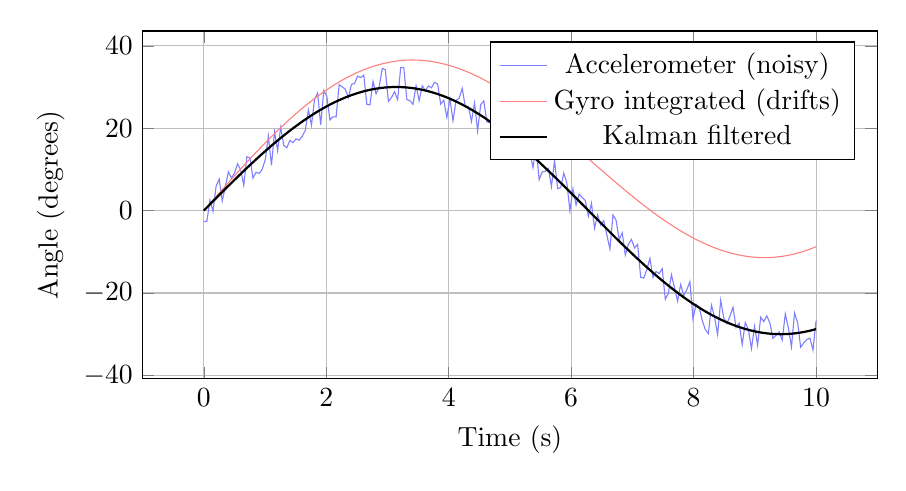
\begin{tikzpicture}
\begin{axis}[
    width=0.9\textwidth,
    height=6cm,
    xlabel={Time (s)},
    ylabel={Angle (degrees)},
    legend pos=north east,
    grid=both,
    domain=0:10,
    samples=200
]

% Simulated noisy accelerometer
\addplot[blue!50, thin] {30*sin(deg(0.5*x)) + 5*rand};
\addlegendentry{Accelerometer (noisy)}

% Simulated drifting gyroscope
\addplot[red!50, thin] {30*sin(deg(0.5*x)) + 2*x};
\addlegendentry{Gyro integrated (drifts)}

% Simulated Kalman filtered
\addplot[black, thick] {30*sin(deg(0.5*x))};
\addlegendentry{Kalman filtered}

\end{axis}
\end{tikzpicture}
\caption{Comparison of sensor measurements and Kalman filter output. The accelerometer (blue) is noisy, the integrated gyroscope (red) drifts over time, while the Kalman filter (black) provides smooth, accurate angle estimates.}
\label{fig:sensor_fusion}
\end{figure}

\section{Worked Examples}

\subsection{Example 1: 1D Position Estimation with Velocity Measurement}

\textbf{Problem:} A vehicle moves along a straight line. We have a noisy position measurement (GPS) and want to estimate both position and velocity.

\textbf{Solution:}

State vector: $\mathbf{x} = \begin{bmatrix} p \\ v \end{bmatrix}$ (position and velocity)

System model (constant velocity with random acceleration):
\begin{equation}
\begin{bmatrix} p_{k+1} \\ v_{k+1} \end{bmatrix} =
\begin{bmatrix} 1 & \Delta t \\ 0 & 1 \end{bmatrix}
\begin{bmatrix} p_k \\ v_k \end{bmatrix} + \mathbf{w}_k
\end{equation}

Measurement model (GPS measures position):
\begin{equation}
y_k = \begin{bmatrix} 1 & 0 \end{bmatrix} \begin{bmatrix} p_k \\ v_k \end{bmatrix} + v_k
\end{equation}

With $\Delta t = 1$ s, $Q = \begin{bmatrix} 0.1 & 0 \\ 0 & 0.1 \end{bmatrix}$, $R = 4$ (GPS noise variance):

\textbf{Step 1: Initialize}
\begin{align}
\hat{\mathbf{x}}_0 &= \begin{bmatrix} 0 \\ 0 \end{bmatrix}, \quad
P_0 = \begin{bmatrix} 10 & 0 \\ 0 & 10 \end{bmatrix}
\end{align}

\textbf{Step 2: Predict for $k=1$}
\begin{align}
\hat{\mathbf{x}}_1^- &= A\hat{\mathbf{x}}_0 = \begin{bmatrix} 1 & 1 \\ 0 & 1 \end{bmatrix}\begin{bmatrix} 0 \\ 0 \end{bmatrix} = \begin{bmatrix} 0 \\ 0 \end{bmatrix} \\
P_1^- &= AP_0A^\top + Q = \begin{bmatrix} 1 & 1 \\ 0 & 1 \end{bmatrix}\begin{bmatrix} 10 & 0 \\ 0 & 10 \end{bmatrix}\begin{bmatrix} 1 & 0 \\ 1 & 1 \end{bmatrix} + \begin{bmatrix} 0.1 & 0 \\ 0 & 0.1 \end{bmatrix} \\
&= \begin{bmatrix} 20.1 & 10 \\ 10 & 10.1 \end{bmatrix}
\end{align}

\textbf{Step 3: Update with measurement $y_1 = 2.5$}
\begin{align}
K_1 &= P_1^-C^\top(CP_1^-C^\top + R)^{-1} \\
&= \begin{bmatrix} 20.1 \\ 10 \end{bmatrix}(20.1 + 4)^{-1} = \begin{bmatrix} 0.834 \\ 0.415 \end{bmatrix}
\end{align}

Innovation: $y_1 - C\hat{\mathbf{x}}_1^- = 2.5 - 0 = 2.5$

\begin{align}
\hat{\mathbf{x}}_1 &= \hat{\mathbf{x}}_1^- + K_1(2.5) = \begin{bmatrix} 0 \\ 0 \end{bmatrix} + \begin{bmatrix} 0.834 \\ 0.415 \end{bmatrix}(2.5) = \begin{bmatrix} 2.08 \\ 1.04 \end{bmatrix}
\end{align}

The filter estimates position at 2.08 m and infers velocity of 1.04 m/s from a single measurement!

\subsection{Example 2: Steady-State Kalman Gain}

\textbf{Problem:} Find the steady-state Kalman gain for a scalar system:
\begin{align}
x_{k+1} &= ax_k + w_k, \quad w_k \sim \mathcal{N}(0, q) \\
y_k &= x_k + v_k, \quad v_k \sim \mathcal{N}(0, r)
\end{align}

\textbf{Solution:}

The discrete algebraic Riccati equation for this scalar system:
\begin{equation}
P = aP a + q - \frac{a^2 P^2}{P + r}
\end{equation}

At steady state, let $P_\infty = P$:
\begin{equation}
P = a^2 P + q - \frac{a^2 P^2}{P + r}
\end{equation}

Multiply by $(P + r)$:
\begin{equation}
P(P + r) = a^2 P(P + r) + q(P + r) - a^2 P^2
\end{equation}

\begin{equation}
P^2 + Pr = a^2 P^2 + a^2 Pr + qP + qr - a^2 P^2
\end{equation}

\begin{equation}
P^2 + Pr = a^2 Pr + qP + qr
\end{equation}

\begin{equation}
P^2 + P(r - a^2 r - q) - qr = 0
\end{equation}

Using the quadratic formula with $a = 0.9$, $q = 0.1$, $r = 1$:
\begin{equation}
P^2 + P(1 - 0.81 - 0.1) - 0.1 = 0 \implies P^2 + 0.09P - 0.1 = 0
\end{equation}

\begin{equation}
P_\infty = \frac{-0.09 + \sqrt{0.0081 + 0.4}}{2} = \frac{-0.09 + 0.639}{2} = 0.274
\end{equation}

Steady-state Kalman gain:
\begin{equation}
K_\infty = \frac{P_\infty}{P_\infty + r} = \frac{0.274}{0.274 + 1} = 0.215
\end{equation}

This means at steady state, the filter weights the measurement at about 21.5\% and the prediction at about 78.5\%.

\subsection{Example 3: Effect of $Q$ and $R$ on Filter Behavior}

\textbf{Problem:} For the system in Example 2, compare the steady-state gain for:
\begin{enumerate}[(a)]
    \item $q = 0.01$, $r = 1$ (trust model more)
    \item $q = 1$, $r = 0.01$ (trust measurements more)
\end{enumerate}

\textbf{Solution:}

\textbf{Case (a):} $q/r = 0.01$ (model-trusting)

Using the same derivation:
\begin{equation}
P^2 + P(1 - 0.81 - 0.01) - 0.01 = 0 \implies P^2 + 0.18P - 0.01 = 0
\end{equation}

$P_\infty = 0.0474$, $K_\infty = \frac{0.0474}{1.0474} = 0.045$

The filter mostly ignores measurements (4.5\% weight).

\textbf{Case (b):} $q/r = 100$ (measurement-trusting)

\begin{equation}
P^2 + P(0.01 - 0.81 \cdot 0.01 - 1) - 0.01 = 0 \implies P^2 - 0.9919P - 0.01 = 0
\end{equation}

$P_\infty = 1.002$, $K_\infty = \frac{1.002}{1.002 + 0.01} = 0.990$

The filter heavily weights measurements (99\% weight).

\subsection{Example 4: Step-by-Step Discrete Kalman Filter}

\textbf{Problem:} Implement three complete cycles of a Kalman filter for tracking a falling object.

\textbf{Setup:}
\begin{align}
A &= \begin{bmatrix} 1 & 0.1 \\ 0 & 1 \end{bmatrix}, \quad
B = \begin{bmatrix} 0.005 \\ 0.1 \end{bmatrix}, \quad
C = \begin{bmatrix} 1 & 0 \end{bmatrix} \\
Q &= \begin{bmatrix} 0.01 & 0 \\ 0 & 0.01 \end{bmatrix}, \quad R = 1
\end{align}

Input $u = -9.81$ (gravity), measurements $y = [0, -0.4, -0.9]$ m.

Initial: $\hat{\mathbf{x}}_0 = [0, 0]^\top$, $P_0 = I$.

\textbf{Solution:}

\textbf{$k = 1$: Predict}
\begin{align}
\hat{\mathbf{x}}_1^- &= A\hat{\mathbf{x}}_0 + Bu = \begin{bmatrix} 0 \\ 0 \end{bmatrix} + \begin{bmatrix} -0.049 \\ -0.981 \end{bmatrix} = \begin{bmatrix} -0.049 \\ -0.981 \end{bmatrix} \\
P_1^- &= AP_0A^\top + Q = \begin{bmatrix} 1.11 & 0.1 \\ 0.1 & 1.01 \end{bmatrix}
\end{align}

\textbf{$k = 1$: Update with $y_1 = 0$}
\begin{align}
S_1 &= CP_1^-C^\top + R = 1.11 + 1 = 2.11 \\
K_1 &= P_1^-C^\top S_1^{-1} = \begin{bmatrix} 0.526 \\ 0.047 \end{bmatrix} \\
\hat{\mathbf{x}}_1 &= \hat{\mathbf{x}}_1^- + K_1(0 - (-0.049)) = \begin{bmatrix} -0.023 \\ -0.978 \end{bmatrix}
\end{align}

Continue this process for $k = 2, 3$ to track the falling object.

\subsection{Example 5: Sensor Fusion---Combining Two Noisy Measurements}

\textbf{Problem:} We have two independent sensors measuring the same quantity $x$:
\begin{align}
y_1 &= x + v_1, \quad v_1 \sim \mathcal{N}(0, \sigma_1^2) \\
y_2 &= x + v_2, \quad v_2 \sim \mathcal{N}(0, \sigma_2^2)
\end{align}

With $\sigma_1 = 2$, $\sigma_2 = 1$, and measurements $y_1 = 10$, $y_2 = 12$, find the optimal estimate.

\textbf{Solution:}

This is a static estimation problem (no dynamics), but we can use Kalman filter concepts.

For scalar independent measurements, the optimal combined estimate is:
\begin{equation}
\hat{x} = \frac{\sigma_2^2 y_1 + \sigma_1^2 y_2}{\sigma_1^2 + \sigma_2^2}
\end{equation}

With our values:
\begin{equation}
\hat{x} = \frac{1 \cdot 10 + 4 \cdot 12}{4 + 1} = \frac{10 + 48}{5} = 11.6
\end{equation}

The combined estimate is closer to $y_2$ because sensor 2 is more accurate (lower variance).

The combined variance is:
\begin{equation}
\sigma_{\text{combined}}^2 = \frac{\sigma_1^2 \sigma_2^2}{\sigma_1^2 + \sigma_2^2} = \frac{4 \cdot 1}{5} = 0.8
\end{equation}

The combined estimate is more accurate than either individual sensor!

\section{Diagrams and Visualizations}

\subsection{Kalman Filter Block Diagram}

\begin{figure}[htbp]
\centering
\begin{tikzpicture}[auto, node distance=2cm, >=latex']
    % Blocks
    \node [block, minimum width=2.5cm] (plant) {Plant};
    \node [block, below=1.5cm of plant, minimum width=2.5cm] (observer) {Kalman Filter};
    \node [sum, left=1.5cm of plant] (sum1) {};
    \node [block, left=1.2cm of sum1] (B) {$B$};
    \node [input, left=1cm of B] (input) {};
    \node [block, right=1.5cm of plant] (C) {$C$};
    \node [sum, right=1cm of C] (sum2) {};
    \node [input, above=0.8cm of sum2] (noise_v) {};
    \node [output, right=1cm of sum2] (output) {};

    % Connections
    \draw [->] (input) -- node {$u$} (B);
    \draw [->] (B) -- (sum1);
    \draw [->] (sum1) -- (plant);
    \draw [->] (plant) -- (C);
    \draw [->] (C) -- (sum2);
    \draw [->] (noise_v) -- node {$v$} (sum2);
    \draw [->] (sum2) -- node {$y$} (output);

    % Process noise
    \node [input, above=0.8cm of sum1] (noise_w) {};
    \draw [->] (noise_w) -- node {$w$} (sum1);

    % Observer feedback
    \draw [->] (sum2) -- ++(0.5,0) |- (observer);
    \draw [->] (observer) -| ++(-3.5,0) |- node[pos=0.8] {$\hat{x}$} ($(sum1)+(-0.5,-0.5)$);

    % Input to observer
    \draw [->] (B) |- ($(observer)+(-2,0)$) -- (observer);

\end{tikzpicture}
\caption{Block diagram of the Kalman filter estimating the state of a plant subject to process noise $w$ and measurement noise $v$.}
\label{fig:kalman_block}
\end{figure}

\subsection{Prediction-Update Cycle}

\begin{figure}[htbp]
\centering
\begin{tikzpicture}[node distance=3cm, auto]
    % Nodes
    \node[draw, rounded corners, fill=blue!20, minimum width=3cm, minimum height=1.5cm] (predict) {
        \begin{tabular}{c}
        \textbf{PREDICT} \\
        $\hat{x}^- = A\hat{x} + Bu$ \\
        $P^- = APA^\top + Q$
        \end{tabular}
    };

    \node[draw, rounded corners, fill=green!20, minimum width=3cm, minimum height=1.5cm, right=2cm of predict] (update) {
        \begin{tabular}{c}
        \textbf{UPDATE} \\
        $K = P^-C^\top(CP^-C^\top + R)^{-1}$ \\
        $\hat{x} = \hat{x}^- + K(y - C\hat{x}^-)$ \\
        $P = (I - KC)P^-$
        \end{tabular}
    };

    % Arrows
    \draw[->, thick] (predict) -- node[above] {$\hat{x}^-, P^-$} (update);
    \draw[->, thick] (update.south) -- ++(0,-1) -| node[below, pos=0.25] {Next time step} (predict.south);

    % Measurement arrow
    \draw[->, thick] ($(update.north)+(0,0.5)$) -- node[right] {$y_k$} (update.north);

\end{tikzpicture}
\caption{The predict-update cycle of the Kalman filter. Each measurement triggers a complete cycle.}
\label{fig:predict_update}
\end{figure}

\subsection{Gaussian Fusion: Prior, Measurement, and Posterior}

\begin{figure}[htbp]
\centering
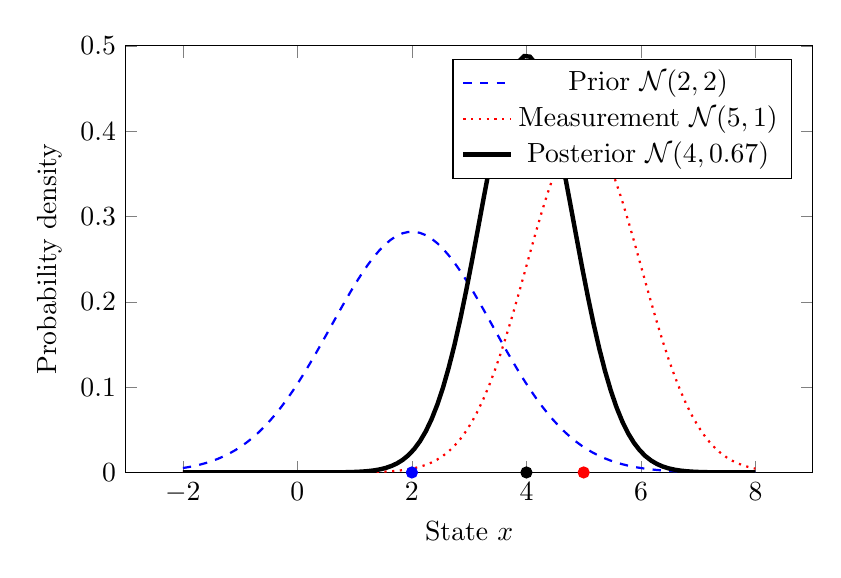
\begin{tikzpicture}
\begin{axis}[
    width=0.85\textwidth,
    height=7cm,
    xlabel={State $x$},
    ylabel={Probability density},
    legend pos=north east,
    domain=-2:8,
    samples=100,
    ymin=0,
    ymax=0.5
]

% Prior distribution (wider, centered at 2)
\addplot[blue, thick, dashed] {exp(-(x-2)^2/(2*2))/(sqrt(2*pi)*sqrt(2))};
\addlegendentry{Prior $\mathcal{N}(2, 2)$}

% Measurement likelihood (narrower, centered at 5)
\addplot[red, thick, dotted] {exp(-(x-5)^2/(2*1))/(sqrt(2*pi)*sqrt(1))};
\addlegendentry{Measurement $\mathcal{N}(5, 1)$}

% Posterior (narrowest, between the two)
\addplot[black, ultra thick] {exp(-(x-4)^2/(2*0.667))/(sqrt(2*pi)*sqrt(0.667))};
\addlegendentry{Posterior $\mathcal{N}(4, 0.67)$}

% Mark the means
\addplot[blue, mark=*, mark size=2pt] coordinates {(2,0)};
\addplot[red, mark=*, mark size=2pt] coordinates {(5,0)};
\addplot[black, mark=*, mark size=2pt] coordinates {(4,0)};

\end{axis}
\end{tikzpicture}
\caption{Bayesian fusion in the Kalman filter. The prior (predicted) distribution is combined with the measurement likelihood to produce the posterior (updated) distribution. The posterior is narrower (more certain) than either input and located between them, weighted by their relative uncertainties.}
\label{fig:gaussian_fusion}
\end{figure}

\subsection{Sensor Comparison: Raw vs. Filtered}

\begin{figure}[htbp]
\centering
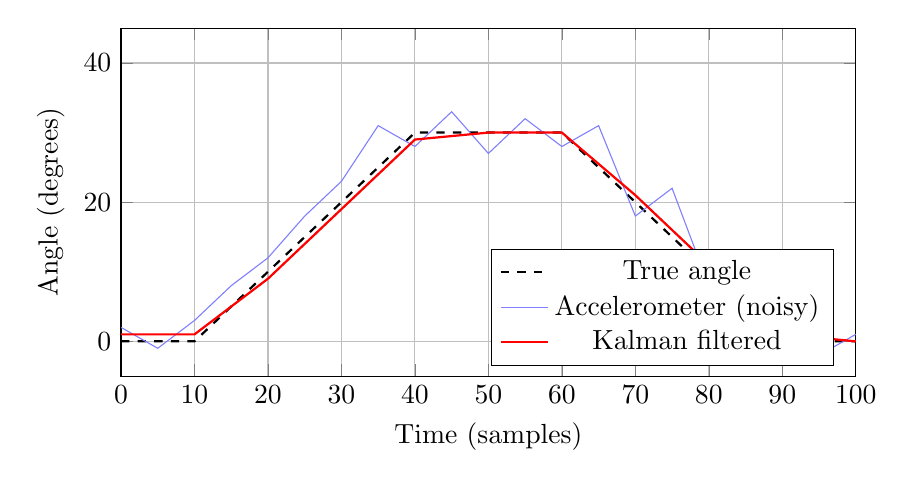
\begin{tikzpicture}
\begin{axis}[
    width=0.9\textwidth,
    height=6cm,
    xlabel={Time (samples)},
    ylabel={Angle (degrees)},
    legend pos=south east,
    grid=both,
    xmin=0, xmax=100,
    ymin=-5, ymax=45
]

% True signal
\addplot[black, thick, dashed] coordinates {
    (0,0) (10,0) (20,10) (30,20) (40,30) (50,30) (60,30) (70,20) (80,10) (90,0) (100,0)
};
\addlegendentry{True angle}

% Noisy accelerometer (simulated)
\addplot[blue!50, thin, mark=none] coordinates {
    (0,2) (5,-1) (10,3) (15,8) (20,12) (25,18) (30,23) (35,31) (40,28) (45,33)
    (50,27) (55,32) (60,28) (65,31) (70,18) (75,22) (80,8) (85,12) (90,3) (95,-2) (100,1)
};
\addlegendentry{Accelerometer (noisy)}

% Kalman filtered
\addplot[red, thick] coordinates {
    (0,1) (10,1) (20,9) (30,19) (40,29) (50,30) (60,30) (70,21) (80,11) (90,1) (100,0)
};
\addlegendentry{Kalman filtered}

\end{axis}
\end{tikzpicture}
\caption{Comparison of raw accelerometer data and Kalman-filtered estimate. The filter tracks the true angle while rejecting high-frequency measurement noise.}
\label{fig:filter_comparison}
\end{figure}

\section{Chapter Summary}

The Kalman filter represents one of the crowning achievements of twentieth-century applied mathematics. By combining optimal estimation theory with recursive computation, Rudolf Kalman solved the fundamental problem of extracting accurate state information from noisy measurements in a computationally tractable way.

\textbf{Key concepts:}
\begin{enumerate}
    \item \textbf{Optimal estimation:} The Kalman filter minimizes mean-square estimation error.

    \item \textbf{Recursive structure:} The filter maintains only a state estimate and error covariance, requiring bounded memory regardless of measurement history length.

    \item \textbf{Predict-update cycle:} Each cycle propagates the estimate forward in time and then corrects it based on new measurements.

    \item \textbf{Kalman gain:} Optimally weights innovation based on relative model and measurement uncertainties.

    \item \textbf{Sensor fusion:} Multiple noisy sensors can be combined to achieve accuracy exceeding any individual sensor.

    \item \textbf{Duality with LQR:} Estimation and control are mathematically dual problems solved by the same Riccati equation structure.
\end{enumerate}

\textbf{Practical considerations:}
\begin{itemize}
    \item Tune $Q$ and $R$ to balance smoothness vs. responsiveness
    \item The filter is optimal only when the linear Gaussian assumptions hold
    \item For nonlinear systems, consider Extended Kalman Filter (EKF) or Unscented Kalman Filter (UKF)
    \item Numerical stability requires care in covariance propagation
\end{itemize}

The Kalman filter's influence extends far beyond control engineering into navigation, signal processing, econometrics, and machine learning. Understanding its principles provides a foundation for the entire field of sequential estimation.

\section{Exercises}

\begin{enumerate}
    \item \textbf{Scalar Kalman filter:} For the system $x_{k+1} = 0.95x_k + w_k$, $y_k = x_k + v_k$ with $Q = 1$ and $R = 10$, compute the steady-state Kalman gain.

    \item \textbf{Prediction without measurement:} If a Kalman filter runs for several time steps without receiving measurements, describe what happens to the error covariance $P$.

    \item \textbf{Observability and Kalman filter:} Explain why an unobservable mode cannot be estimated by the Kalman filter.

    \item \textbf{Tuning trade-offs:} A tracking filter follows a maneuvering target. Should $Q$ be set high or low? Justify your answer.

    \item \textbf{IMU fusion derivation:} Derive the complete state-space model for fusing accelerometer and gyroscope measurements to estimate pitch and roll angles.

    \item \textbf{Numerical experiment:} Implement the discrete Kalman filter in MATLAB/Python for a double integrator (position from noisy velocity measurements). Plot the estimation error versus time for various $Q/R$ ratios.

    \item \textbf{Innovation sequence:} The innovation sequence $\nu_k = y_k - C\hat{x}_k^-$ should be white noise if the filter is correctly tuned. Design an experiment to test this property.

    \item \textbf{Joseph form:} The covariance update $P = (I-KC)P^-$ can suffer from numerical issues. Research and explain the ``Joseph form'' update and why it is more numerically stable.
\end{enumerate}

\section{Further Reading}

\begin{enumerate}
    \item Kalman, R.E. (1960). ``A New Approach to Linear Filtering and Prediction Problems.'' \textit{Journal of Basic Engineering}, 82(1), 35--45. \textit{The original paper---remarkably readable.}

    \item Brown, R.G. and Hwang, P.Y.C. (2012). \textit{Introduction to Random Signals and Applied Kalman Filtering}. Wiley. \textit{Excellent practical introduction.}

    \item Simon, D. (2006). \textit{Optimal State Estimation: Kalman, H$\infty$, and Nonlinear Approaches}. Wiley. \textit{Comprehensive modern treatment.}

    \item Grewal, M.S. and Andrews, A.P. (2015). \textit{Kalman Filtering: Theory and Practice Using MATLAB}. Wiley. \textit{Implementation-focused.}

    \item McGee, L.A. and Schmidt, S.F. (1985). ``Discovery of the Kalman Filter as a Practical Tool for Aerospace and Industry.'' NASA TM-86847. \textit{Fascinating historical account by the NASA engineers who first implemented it.}
\end{enumerate}

\begin{thebibliography}{9}
\bibitem{kalman1960}
R.E. Kalman, ``A New Approach to Linear Filtering and Prediction Problems,'' \textit{Journal of Basic Engineering}, vol. 82, no. 1, pp. 35--45, 1960.
\end{thebibliography}
